\chapter{Conversion statique de puissance}
\thispagestyle{plain} % Supprimer le header & le footer sur cette page en laissant la numérotation
\newpage

%----------------------------------------------------------------------------------------
%	Les hacheurs
%----------------------------------------------------------------------------------------

\section{Les montages hacheur}

\exercice{Étude montage hacheur série ou dévolteur}
Le hacheur série de la figure ci-dessous alimente une charge constituée par une inductance $L$ de $20mH$ en série avec un moteur dont la fem est $E’=99V$ lorsque le rapport cyclique $\alpha$ est de $0,792$. On néglige la résistance de la source de sortie et la source d’entrée a une fem $E$  constante dans tout le problème. La fréquence de hachage est de $f=2,5kHz$ et le courant moyen est de $6A$.
\begin{center}
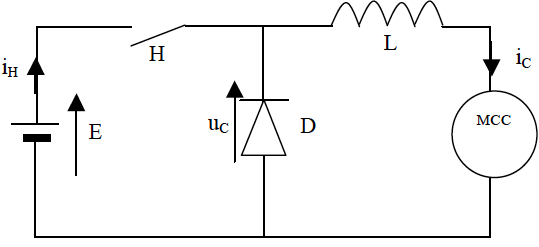
\includegraphics[scale=0.5]{png/hacheur1.png}
\end{center}

\subsubsection{Travail demandé}
\begin{enumerate}
\item Tracer l’allure de $U_C(t)$ au cours d’une période de fonctionnement. 
\item Calculer la valeur de la fem $E$ de la source. 
\item Tracer l’allure du courant dans la charge en fonction du temps. 
\item Quelle est la valeur de l’ondulation du courant $\Delta I_C$ dans la charge ? En déduire la valeur maximale de cette ondulation et pour quelle valeur du rapport cyclique est elle obtenue ? \\
En supposant que la fem de la machine à courant continu reste constante ainsi que la valeur moyenne du courant d’induit, on fait varier la fréquence de hachage à rapport cyclique constant.
\item On souhaite se placer à la limite du fonctionnement continu. Quelle est la valeur maximale du courant $I_C$ correspondante ?
\item Pour quelle valeur de la fréquence obtient on la limite de fonctionnement continu ? 
\end{enumerate}



\correction{ % Answer
\begin{enumerate}
\item $U_C=E$ de $0$ à $\alpha.T$, nulle ailleurs;
\item Comme $E'=\alpha E$, on obtient $E=\frac{E'}{\alpha}=125V$; 
\item On suppose à $t=0$, $i_c(t=0)=i_0$. Comme $i_c(t=0)=\frac{1}{L} \int_0^T U_L dt$.\\
Pour $t \in [0,\alpha T[$, $U_L=E'-E=(1-\alpha)E$ d'où \fbox{$i_c(t)=i_0+\frac{(1-\alpha)E}{L}t$}.\\
On a alors \fbox{$i_{max}=i_0+\frac{(1-\alpha)E}{L}T=0,63A$}\\
Pour $t \in [\alpha T, T[$, $U_L=-E'=-\alpha)E$ d'où \fbox{$i_c(t)=i_{max}-\frac{-\alpha E}{L}(t-\alpha T)$}.
\item On en déduit $\Delta I_C=i_{max}-i_0$, \fbox{$\Delta I_C=\frac{1-\alpha}{L}E \alpha T$}\\
L'ondulation est maximale lorsque $\frac{\delta \Delta I_C}{\delta \alpha}=0$ d'où $\alpha=\frac{1}{2}$. Ainsi $\Delta I_{Cmax}=0,625$
\item $\Delta I_C=I_{limite}=2<I_C>$ d'où $I_{limite}=12A$
\item $\Delta I_C=I_{limite}$ implique que $\frac{1-\alpha}{L}E \alpha \frac{1}{f} =I_{limite}$ d'où \fbox{$f=\frac{1-\alpha}{L I_{limite}}E \alpha=85,8kHz$}
\end{enumerate}
}
\newpage

%--------------------------------------------

\exercice{Étude d’un montage hacheur parallèle }
Soit le montage fourni ci-dessous où $H$ désigne un interrupteur parfait commandable à l’ouverture et à la fermeture. On se place en régime permanent de fonctionnement : 
\begin{center}
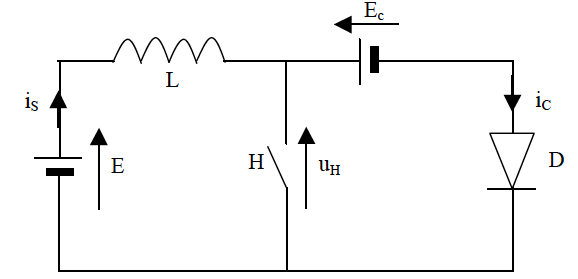
\includegraphics[scale=0.5]{png/hacheur2.png}
\end{center}
de $t_0=0$ à $t_1=\frac{2T}{3}$ : $H$ est fermé;\\
de $t_1=\frac{2T}{3}$ à $t_2=T$ : $H$ est ouvert.\\
On précise les valeurs des composants et de la période : $E=48V$ ; $L=25mH$ ; $T=0,5ms$.

\subsubsection{Travail demandé}
\begin{enumerate}
\item Quel est l’état de la diode $D$ lorsque $H$ est fermé ?
\item Comment évolue le courant $i_s(t)$ durant cette phase ? On supposera connue la valeur du courant à l’instant $t_0=0$ : $i_s(t=0)=I_{min}=12A$.
\item Lorsque l’interrupteur $H$ est ouvert, que vaut la tension $u_H$ ? Représenter les allures de $u_H$ et de $i_s(t)$ pour l’intervalle $t_1$ à $t_2$.
\item Exprimer la valeur moyenne de la tension aux bornes de $H$, et en déduire la valeur de $E_c$.
\item Calculer l’ondulation de $i_s$. Quelle est sa valeur maximum ?  
\end{enumerate}


\correction{ % Answer
\begin{enumerate}
\item $H$ fermé. d'où $U_D=-E_c$. Donc \fbox{$D$ bloquante}
\item \(i_s(t)=\frac{1}{L}\int U_L dt\). Comme $H$ fermé, $U_L=E$.\\
On a alors \fbox{\(i_s(t)=I_{min} + \frac{E}{L}t=12+1920t \)}
\item \fbox{\( U_H=E_c\) pour $t\in [t_1,t_2[$, sinon nulle}\\
Pour $t\in [0,t_1[$, \(i_s(t)=I_{min} + \frac{E}{L}t\) (question précédente)
Pour $t\in [t_1,t_2[$, $U_L=E-E_c<0$ d'où \fbox{\(i_s(t)=I_{max} + \frac{E-E_c}{L}t\)}
\item $U_H=(1-\alpha)E_c$ (visible graphiquement). Comme $u_H(t)+L\frac{di_s}{dt}=E$, $U_H=E$.\\
Ainsi \fbox{\(E_c=\frac{E}{1-\alpha}=144V \)}
\item Comme \( \Delta i_s=I_{max}-I_{min} \), \fbox{\(\Delta i_s=\frac{E \alpha T}{L} \)}
\end{enumerate}
}
\newpage

%--------------------------------------------

\exercice{Étude d’un montage hacheur inverseur à stockage inductif }
Le montage de la figure ci-dessous est un convertisseur statique indirect. Il fonctionne en régime permanent par l’intermédiaire de l’interrupteur $H$, unidirectionnel en courant, commandé à l’ouverture et à la fermeture de façon périodique, supposé parfait. 
\begin{center}
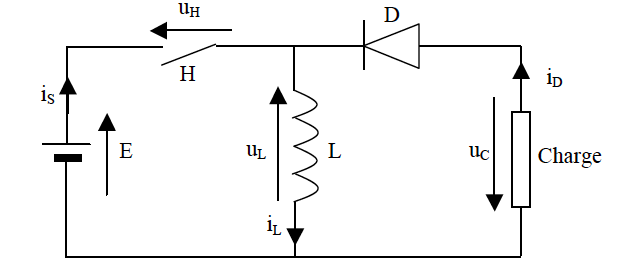
\includegraphics[scale=0.5]{png/hacheur3.png}
\end{center}

de $t_0=0$ à $t_1=\alpha.T$ : $H$ est fermé ;
de $t_1$ à $t_2=T$ : $H$ est ouvert.

On précise les valeurs des composants : $E=48V$ ; $L=25mH$ ; la charge est constituée par la mise en parallèle d’une résistance $R=100.\Omega$ et d’un condensateur de capacité $C=1000 \mu F$ imposant une tension $u_C$ constante pour un rapport cyclique imposé constant. La période de hachage est de $T=500 \mu s$. La diode $D$ est supposée parfaite.

\subsubsection{Travail demandé}
\begin{enumerate}
\item Quel est l’état de la diode $D$ lorsque $H$ est fermé ? 
\item Comment évolue $i_s$ lorsque $H$ est fermé ? On notera $I_0$ sa valeur à $t_0$. 
\item Lorsque $H$ est ouvert, que vaut le courant $i_L$ ? Comment évolue t’il ? 
\item Représenter $u_L$, $u_H$ et $i_L$ sur une période. 
\item Calculer l’ondulation du courant sur une période pour $\alpha=\frac{1}{3}$ et $\frac{2}{3}$. 
\item Exprimer $<u_C>$  en fonction de $E$ et du rapport cyclique $\alpha$. 
\item Calculer numériquement la valeur moyenne de $u_C$ pour un rapport cyclique de $\frac{1}{3}$ et $\frac{2}{3}$.
\item Pour un rapport cyclique de $\frac{1}{3}$ et pour$\frac{2}{3}$, évaluer le courant dans la charge et la puissance délivrée à celle-ci. 
\end{enumerate}


\correction{ % Answer
\begin{enumerate}
\item Comme $H$ est fermé, $U_L=E$ d'où $U_D=U_L+U_c>0$.\\ Donc \fbox{D est bloquée.}
\item Comme $H$ est fermé, $U_L=E$.\\
Or $i_s(t)=\frac{1}{L}\int u_L(t) dt$ d'où \fbox{$i_s(t)=I_0+\frac{E}{L}t$}
\item Comme $H$ est ouvert, $U_L=-U_c$.\\
\fbox{$i_L(t)=I_1-U_c.\frac{(t-\alpha.T)}{L}$ avec $I_1=I_0+\frac{E}{L}\alpha T$}
\item GRAPHES
\item \fbox{$\Delta I_L=I_1-I_0=\frac{E\alpha T}{L}$}\\
Pour $\alpha=\frac{1}{3}$, $\Delta I_L=32mA$\\
Pour $\alpha=\frac{2}{3}$, $\Delta I_L=64mA$.
\item $<U_L>=\alpha E.T-(1-\alpha)T.U_c =0$ (Graphiquement) d'où \fbox{$U_c=\frac{\alpha}{1-\alpha}E$}
\item Pour $\alpha=\frac{1}{3}$, $U_c=24V$\\
Pour $\alpha=\frac{2}{3}$, $U_c=96V$.
\item \fbox{$P=\frac{U_c^{2}}{R}$ et $I_c=\frac{U_c}{R}$}
Pour $\alpha=\frac{1}{3}$, $I_c=240mA$ et $P=5,76W$\\
Pour $\alpha=\frac{2}{3}$, $I_c=960mA$ et $P=92W$.

\end{enumerate}
}
\newpage

%--------------------------------------------